% Created by tikzDevice version 0.12
% !TEX encoding = UTF-8 Unicode
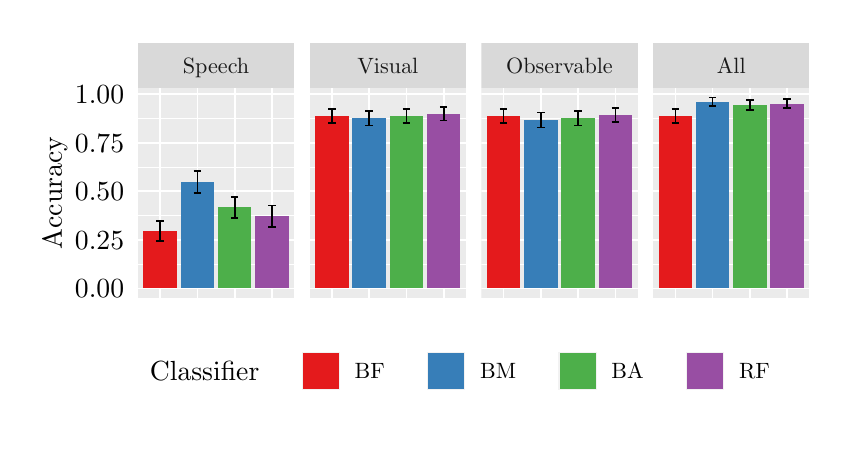
\begin{tikzpicture}[x=1pt,y=1pt]
\definecolor{fillColor}{RGB}{255,255,255}
\path[use as bounding box,fill=fillColor,fill opacity=0.00] (0,0) rectangle (288.00,142.39);
\begin{scope}
\path[clip] (  0.00,  0.00) rectangle (288.00,142.39);
\definecolor{drawColor}{RGB}{255,255,255}
\definecolor{fillColor}{RGB}{255,255,255}

\path[draw=drawColor,line width= 0.6pt,line join=round,line cap=round,fill=fillColor] (  0.00,  0.00) rectangle (288.00,142.39);
\end{scope}
\begin{scope}
\path[clip] ( 39.80, 44.70) rectangle ( 96.35,120.63);
\definecolor{fillColor}{gray}{0.92}

\path[fill=fillColor] ( 39.80, 44.70) rectangle ( 96.35,120.63);
\definecolor{drawColor}{RGB}{255,255,255}

\path[draw=drawColor,line width= 0.3pt,line join=round] ( 39.80, 56.93) --
	( 96.35, 56.93);

\path[draw=drawColor,line width= 0.3pt,line join=round] ( 39.80, 74.49) --
	( 96.35, 74.49);

\path[draw=drawColor,line width= 0.3pt,line join=round] ( 39.80, 92.04) --
	( 96.35, 92.04);

\path[draw=drawColor,line width= 0.3pt,line join=round] ( 39.80,109.60) --
	( 96.35,109.60);

\path[draw=drawColor,line width= 0.6pt,line join=round] ( 39.80, 48.16) --
	( 96.35, 48.16);

\path[draw=drawColor,line width= 0.6pt,line join=round] ( 39.80, 65.71) --
	( 96.35, 65.71);

\path[draw=drawColor,line width= 0.6pt,line join=round] ( 39.80, 83.27) --
	( 96.35, 83.27);

\path[draw=drawColor,line width= 0.6pt,line join=round] ( 39.80,100.82) --
	( 96.35,100.82);

\path[draw=drawColor,line width= 0.6pt,line join=round] ( 39.80,118.38) --
	( 96.35,118.38);

\path[draw=drawColor,line width= 0.6pt,line join=round] ( 47.88, 44.70) --
	( 47.88,120.63);

\path[draw=drawColor,line width= 0.6pt,line join=round] ( 61.35, 44.70) --
	( 61.35,120.63);

\path[draw=drawColor,line width= 0.6pt,line join=round] ( 74.81, 44.70) --
	( 74.81,120.63);

\path[draw=drawColor,line width= 0.6pt,line join=round] ( 88.28, 44.70) --
	( 88.28,120.63);
\definecolor{fillColor}{RGB}{228,26,28}

\path[fill=fillColor] ( 41.82, 48.16) rectangle ( 53.94, 68.94);
\definecolor{fillColor}{RGB}{55,126,184}

\path[fill=fillColor] ( 55.29, 48.16) rectangle ( 67.41, 86.57);
\definecolor{fillColor}{RGB}{77,175,74}

\path[fill=fillColor] ( 68.75, 48.16) rectangle ( 80.87, 77.44);
\definecolor{fillColor}{RGB}{152,78,163}

\path[fill=fillColor] ( 82.22, 48.16) rectangle ( 94.33, 74.21);
\definecolor{drawColor}{RGB}{0,0,0}

\path[draw=drawColor,line width= 0.6pt,line join=round] ( 46.54, 72.59) --
	( 49.23, 72.59);

\path[draw=drawColor,line width= 0.6pt,line join=round] ( 47.88, 72.59) --
	( 47.88, 65.36);

\path[draw=drawColor,line width= 0.6pt,line join=round] ( 46.54, 65.36) --
	( 49.23, 65.36);

\path[draw=drawColor,line width= 0.6pt,line join=round] ( 60.00, 90.50) --
	( 62.69, 90.50);

\path[draw=drawColor,line width= 0.6pt,line join=round] ( 61.35, 90.50) --
	( 61.35, 82.63);

\path[draw=drawColor,line width= 0.6pt,line join=round] ( 60.00, 82.63) --
	( 62.69, 82.63);

\path[draw=drawColor,line width= 0.6pt,line join=round] ( 73.46, 81.30) --
	( 76.16, 81.30);

\path[draw=drawColor,line width= 0.6pt,line join=round] ( 74.81, 81.30) --
	( 74.81, 73.50);

\path[draw=drawColor,line width= 0.6pt,line join=round] ( 73.46, 73.50) --
	( 76.16, 73.50);

\path[draw=drawColor,line width= 0.6pt,line join=round] ( 86.93, 78.07) --
	( 89.62, 78.07);

\path[draw=drawColor,line width= 0.6pt,line join=round] ( 88.28, 78.07) --
	( 88.28, 70.42);

\path[draw=drawColor,line width= 0.6pt,line join=round] ( 86.93, 70.42) --
	( 89.62, 70.42);
\end{scope}
\begin{scope}
\path[clip] (101.85, 44.70) rectangle (158.40,120.63);
\definecolor{fillColor}{gray}{0.92}

\path[fill=fillColor] (101.85, 44.70) rectangle (158.40,120.63);
\definecolor{drawColor}{RGB}{255,255,255}

\path[draw=drawColor,line width= 0.3pt,line join=round] (101.85, 56.93) --
	(158.40, 56.93);

\path[draw=drawColor,line width= 0.3pt,line join=round] (101.85, 74.49) --
	(158.40, 74.49);

\path[draw=drawColor,line width= 0.3pt,line join=round] (101.85, 92.04) --
	(158.40, 92.04);

\path[draw=drawColor,line width= 0.3pt,line join=round] (101.85,109.60) --
	(158.40,109.60);

\path[draw=drawColor,line width= 0.6pt,line join=round] (101.85, 48.16) --
	(158.40, 48.16);

\path[draw=drawColor,line width= 0.6pt,line join=round] (101.85, 65.71) --
	(158.40, 65.71);

\path[draw=drawColor,line width= 0.6pt,line join=round] (101.85, 83.27) --
	(158.40, 83.27);

\path[draw=drawColor,line width= 0.6pt,line join=round] (101.85,100.82) --
	(158.40,100.82);

\path[draw=drawColor,line width= 0.6pt,line join=round] (101.85,118.38) --
	(158.40,118.38);

\path[draw=drawColor,line width= 0.6pt,line join=round] (109.93, 44.70) --
	(109.93,120.63);

\path[draw=drawColor,line width= 0.6pt,line join=round] (123.40, 44.70) --
	(123.40,120.63);

\path[draw=drawColor,line width= 0.6pt,line join=round] (136.86, 44.70) --
	(136.86,120.63);

\path[draw=drawColor,line width= 0.6pt,line join=round] (150.32, 44.70) --
	(150.32,120.63);
\definecolor{fillColor}{RGB}{228,26,28}

\path[fill=fillColor] (103.87, 48.16) rectangle (115.99,110.37);
\definecolor{fillColor}{RGB}{55,126,184}

\path[fill=fillColor] (117.34, 48.16) rectangle (129.45,109.67);
\definecolor{fillColor}{RGB}{77,175,74}

\path[fill=fillColor] (130.80, 48.16) rectangle (142.92,110.37);
\definecolor{fillColor}{RGB}{152,78,163}

\path[fill=fillColor] (144.27, 48.16) rectangle (156.38,111.28);
\definecolor{drawColor}{RGB}{0,0,0}

\path[draw=drawColor,line width= 0.6pt,line join=round] (108.59,112.90) --
	(111.28,112.90);

\path[draw=drawColor,line width= 0.6pt,line join=round] (109.93,112.90) --
	(109.93,107.84);

\path[draw=drawColor,line width= 0.6pt,line join=round] (108.59,107.84) --
	(111.28,107.84);

\path[draw=drawColor,line width= 0.6pt,line join=round] (122.05,112.27) --
	(124.74,112.27);

\path[draw=drawColor,line width= 0.6pt,line join=round] (123.40,112.27) --
	(123.40,107.07);

\path[draw=drawColor,line width= 0.6pt,line join=round] (122.05,107.07) --
	(124.74,107.07);

\path[draw=drawColor,line width= 0.6pt,line join=round] (135.51,112.90) --
	(138.21,112.90);

\path[draw=drawColor,line width= 0.6pt,line join=round] (136.86,112.90) --
	(136.86,107.84);

\path[draw=drawColor,line width= 0.6pt,line join=round] (135.51,107.84) --
	(138.21,107.84);

\path[draw=drawColor,line width= 0.6pt,line join=round] (148.98,113.67) --
	(151.67,113.67);

\path[draw=drawColor,line width= 0.6pt,line join=round] (150.32,113.67) --
	(150.32,108.90);

\path[draw=drawColor,line width= 0.6pt,line join=round] (148.98,108.90) --
	(151.67,108.90);
\end{scope}
\begin{scope}
\path[clip] (163.90, 44.70) rectangle (220.45,120.63);
\definecolor{fillColor}{gray}{0.92}

\path[fill=fillColor] (163.90, 44.70) rectangle (220.45,120.63);
\definecolor{drawColor}{RGB}{255,255,255}

\path[draw=drawColor,line width= 0.3pt,line join=round] (163.90, 56.93) --
	(220.45, 56.93);

\path[draw=drawColor,line width= 0.3pt,line join=round] (163.90, 74.49) --
	(220.45, 74.49);

\path[draw=drawColor,line width= 0.3pt,line join=round] (163.90, 92.04) --
	(220.45, 92.04);

\path[draw=drawColor,line width= 0.3pt,line join=round] (163.90,109.60) --
	(220.45,109.60);

\path[draw=drawColor,line width= 0.6pt,line join=round] (163.90, 48.16) --
	(220.45, 48.16);

\path[draw=drawColor,line width= 0.6pt,line join=round] (163.90, 65.71) --
	(220.45, 65.71);

\path[draw=drawColor,line width= 0.6pt,line join=round] (163.90, 83.27) --
	(220.45, 83.27);

\path[draw=drawColor,line width= 0.6pt,line join=round] (163.90,100.82) --
	(220.45,100.82);

\path[draw=drawColor,line width= 0.6pt,line join=round] (163.90,118.38) --
	(220.45,118.38);

\path[draw=drawColor,line width= 0.6pt,line join=round] (171.98, 44.70) --
	(171.98,120.63);

\path[draw=drawColor,line width= 0.6pt,line join=round] (185.44, 44.70) --
	(185.44,120.63);

\path[draw=drawColor,line width= 0.6pt,line join=round] (198.91, 44.70) --
	(198.91,120.63);

\path[draw=drawColor,line width= 0.6pt,line join=round] (212.37, 44.70) --
	(212.37,120.63);
\definecolor{fillColor}{RGB}{228,26,28}

\path[fill=fillColor] (165.92, 48.16) rectangle (178.04,110.37);
\definecolor{fillColor}{RGB}{55,126,184}

\path[fill=fillColor] (179.39, 48.16) rectangle (191.50,108.97);
\definecolor{fillColor}{RGB}{77,175,74}

\path[fill=fillColor] (192.85, 48.16) rectangle (204.97,109.67);
\definecolor{fillColor}{RGB}{152,78,163}

\path[fill=fillColor] (206.31, 48.16) rectangle (218.43,110.86);
\definecolor{drawColor}{RGB}{0,0,0}

\path[draw=drawColor,line width= 0.6pt,line join=round] (170.63,112.90) --
	(173.33,112.90);

\path[draw=drawColor,line width= 0.6pt,line join=round] (171.98,112.90) --
	(171.98,107.84);

\path[draw=drawColor,line width= 0.6pt,line join=round] (170.63,107.84) --
	(173.33,107.84);

\path[draw=drawColor,line width= 0.6pt,line join=round] (184.10,111.70) --
	(186.79,111.70);

\path[draw=drawColor,line width= 0.6pt,line join=round] (185.44,111.70) --
	(185.44,106.30);

\path[draw=drawColor,line width= 0.6pt,line join=round] (184.10,106.30) --
	(186.79,106.30);

\path[draw=drawColor,line width= 0.6pt,line join=round] (197.56,112.27) --
	(200.26,112.27);

\path[draw=drawColor,line width= 0.6pt,line join=round] (198.91,112.27) --
	(198.91,107.07);

\path[draw=drawColor,line width= 0.6pt,line join=round] (197.56,107.07) --
	(200.26,107.07);

\path[draw=drawColor,line width= 0.6pt,line join=round] (211.03,113.25) --
	(213.72,113.25);

\path[draw=drawColor,line width= 0.6pt,line join=round] (212.37,113.25) --
	(212.37,108.40);

\path[draw=drawColor,line width= 0.6pt,line join=round] (211.03,108.40) --
	(213.72,108.40);
\end{scope}
\begin{scope}
\path[clip] (225.95, 44.70) rectangle (282.50,120.63);
\definecolor{fillColor}{gray}{0.92}

\path[fill=fillColor] (225.95, 44.70) rectangle (282.50,120.63);
\definecolor{drawColor}{RGB}{255,255,255}

\path[draw=drawColor,line width= 0.3pt,line join=round] (225.95, 56.93) --
	(282.50, 56.93);

\path[draw=drawColor,line width= 0.3pt,line join=round] (225.95, 74.49) --
	(282.50, 74.49);

\path[draw=drawColor,line width= 0.3pt,line join=round] (225.95, 92.04) --
	(282.50, 92.04);

\path[draw=drawColor,line width= 0.3pt,line join=round] (225.95,109.60) --
	(282.50,109.60);

\path[draw=drawColor,line width= 0.6pt,line join=round] (225.95, 48.16) --
	(282.50, 48.16);

\path[draw=drawColor,line width= 0.6pt,line join=round] (225.95, 65.71) --
	(282.50, 65.71);

\path[draw=drawColor,line width= 0.6pt,line join=round] (225.95, 83.27) --
	(282.50, 83.27);

\path[draw=drawColor,line width= 0.6pt,line join=round] (225.95,100.82) --
	(282.50,100.82);

\path[draw=drawColor,line width= 0.6pt,line join=round] (225.95,118.38) --
	(282.50,118.38);

\path[draw=drawColor,line width= 0.6pt,line join=round] (234.03, 44.70) --
	(234.03,120.63);

\path[draw=drawColor,line width= 0.6pt,line join=round] (247.49, 44.70) --
	(247.49,120.63);

\path[draw=drawColor,line width= 0.6pt,line join=round] (260.96, 44.70) --
	(260.96,120.63);

\path[draw=drawColor,line width= 0.6pt,line join=round] (274.42, 44.70) --
	(274.42,120.63);
\definecolor{fillColor}{RGB}{228,26,28}

\path[fill=fillColor] (227.97, 48.16) rectangle (240.09,110.37);
\definecolor{fillColor}{RGB}{55,126,184}

\path[fill=fillColor] (241.43, 48.16) rectangle (253.55,115.64);
\definecolor{fillColor}{RGB}{77,175,74}

\path[fill=fillColor] (254.90, 48.16) rectangle (267.02,114.51);
\definecolor{fillColor}{RGB}{152,78,163}

\path[fill=fillColor] (268.36, 48.16) rectangle (280.48,114.94);
\definecolor{drawColor}{RGB}{0,0,0}

\path[draw=drawColor,line width= 0.6pt,line join=round] (232.68,112.90) --
	(235.38,112.90);

\path[draw=drawColor,line width= 0.6pt,line join=round] (234.03,112.90) --
	(234.03,107.84);

\path[draw=drawColor,line width= 0.6pt,line join=round] (232.68,107.84) --
	(235.38,107.84);

\path[draw=drawColor,line width= 0.6pt,line join=round] (246.15,117.18) --
	(248.84,117.18);

\path[draw=drawColor,line width= 0.6pt,line join=round] (247.49,117.18) --
	(247.49,114.09);

\path[draw=drawColor,line width= 0.6pt,line join=round] (246.15,114.09) --
	(248.84,114.09);

\path[draw=drawColor,line width= 0.6pt,line join=round] (259.61,116.27) --
	(262.30,116.27);

\path[draw=drawColor,line width= 0.6pt,line join=round] (260.96,116.27) --
	(260.96,112.69);

\path[draw=drawColor,line width= 0.6pt,line join=round] (259.61,112.69) --
	(262.30,112.69);

\path[draw=drawColor,line width= 0.6pt,line join=round] (273.08,116.62) --
	(275.77,116.62);

\path[draw=drawColor,line width= 0.6pt,line join=round] (274.42,116.62) --
	(274.42,113.25);

\path[draw=drawColor,line width= 0.6pt,line join=round] (273.08,113.25) --
	(275.77,113.25);
\end{scope}
\begin{scope}
\path[clip] ( 39.80,120.63) rectangle ( 96.35,136.89);
\definecolor{fillColor}{gray}{0.85}

\path[fill=fillColor] ( 39.80,120.63) rectangle ( 96.35,136.89);
\definecolor{drawColor}{gray}{0.10}

\node[text=drawColor,anchor=base,inner sep=0pt, outer sep=0pt, scale=  0.80] at ( 68.08,126.01) {Speech};
\end{scope}
\begin{scope}
\path[clip] (101.85,120.63) rectangle (158.40,136.89);
\definecolor{fillColor}{gray}{0.85}

\path[fill=fillColor] (101.85,120.63) rectangle (158.40,136.89);
\definecolor{drawColor}{gray}{0.10}

\node[text=drawColor,anchor=base,inner sep=0pt, outer sep=0pt, scale=  0.80] at (130.13,126.01) {Visual};
\end{scope}
\begin{scope}
\path[clip] (163.90,120.63) rectangle (220.45,136.89);
\definecolor{fillColor}{gray}{0.85}

\path[fill=fillColor] (163.90,120.63) rectangle (220.45,136.89);
\definecolor{drawColor}{gray}{0.10}

\node[text=drawColor,anchor=base,inner sep=0pt, outer sep=0pt, scale=  0.80] at (192.18,126.01) {Observable};
\end{scope}
\begin{scope}
\path[clip] (225.95,120.63) rectangle (282.50,136.89);
\definecolor{fillColor}{gray}{0.85}

\path[fill=fillColor] (225.95,120.63) rectangle (282.50,136.89);
\definecolor{drawColor}{gray}{0.10}

\node[text=drawColor,anchor=base,inner sep=0pt, outer sep=0pt, scale=  0.80] at (254.23,126.01) {All};
\end{scope}
\begin{scope}
\path[clip] (  0.00,  0.00) rectangle (288.00,142.39);
\definecolor{drawColor}{RGB}{0,0,0}

\node[text=drawColor,anchor=base east,inner sep=0pt, outer sep=0pt, scale=  1.00] at ( 34.85, 44.71) {0.00};

\node[text=drawColor,anchor=base east,inner sep=0pt, outer sep=0pt, scale=  1.00] at ( 34.85, 62.27) {0.25};

\node[text=drawColor,anchor=base east,inner sep=0pt, outer sep=0pt, scale=  1.00] at ( 34.85, 79.82) {0.50};

\node[text=drawColor,anchor=base east,inner sep=0pt, outer sep=0pt, scale=  1.00] at ( 34.85, 97.38) {0.75};

\node[text=drawColor,anchor=base east,inner sep=0pt, outer sep=0pt, scale=  1.00] at ( 34.85,114.93) {1.00};
\end{scope}
\begin{scope}
\path[clip] (  0.00,  0.00) rectangle (288.00,142.39);
\definecolor{drawColor}{RGB}{0,0,0}

\node[text=drawColor,rotate= 90.00,anchor=base,inner sep=0pt, outer sep=0pt, scale=  1.00] at ( 12.39, 82.67) {Accuracy};
\end{scope}
\begin{scope}
\path[clip] (  0.00,  0.00) rectangle (288.00,142.39);
\definecolor{fillColor}{RGB}{255,255,255}

\path[fill=fillColor] ( 38.63,  5.50) rectangle (283.67, 30.95);
\end{scope}
\begin{scope}
\path[clip] (  0.00,  0.00) rectangle (288.00,142.39);
\definecolor{drawColor}{RGB}{0,0,0}

\node[text=drawColor,anchor=base west,inner sep=0pt, outer sep=0pt, scale=  1.00] at ( 44.13, 14.78) {Classifier};
\end{scope}
\begin{scope}
\path[clip] (  0.00,  0.00) rectangle (288.00,142.39);
\definecolor{drawColor}{RGB}{255,255,255}
\definecolor{fillColor}{gray}{0.95}

\path[draw=drawColor,line width= 0.6pt,line join=round,line cap=round,fill=fillColor] ( 98.70, 11.00) rectangle (113.16, 25.45);
\end{scope}
\begin{scope}
\path[clip] (  0.00,  0.00) rectangle (288.00,142.39);
\definecolor{fillColor}{RGB}{228,26,28}

\path[fill=fillColor] ( 99.41, 11.71) rectangle (112.45, 24.74);
\end{scope}
\begin{scope}
\path[clip] (  0.00,  0.00) rectangle (288.00,142.39);
\definecolor{drawColor}{RGB}{255,255,255}
\definecolor{fillColor}{gray}{0.95}

\path[draw=drawColor,line width= 0.6pt,line join=round,line cap=round,fill=fillColor] (144.04, 11.00) rectangle (158.50, 25.45);
\end{scope}
\begin{scope}
\path[clip] (  0.00,  0.00) rectangle (288.00,142.39);
\definecolor{fillColor}{RGB}{55,126,184}

\path[fill=fillColor] (144.76, 11.71) rectangle (157.79, 24.74);
\end{scope}
\begin{scope}
\path[clip] (  0.00,  0.00) rectangle (288.00,142.39);
\definecolor{drawColor}{RGB}{255,255,255}
\definecolor{fillColor}{gray}{0.95}

\path[draw=drawColor,line width= 0.6pt,line join=round,line cap=round,fill=fillColor] (191.49, 11.00) rectangle (205.95, 25.45);
\end{scope}
\begin{scope}
\path[clip] (  0.00,  0.00) rectangle (288.00,142.39);
\definecolor{fillColor}{RGB}{77,175,74}

\path[fill=fillColor] (192.21, 11.71) rectangle (205.24, 24.74);
\end{scope}
\begin{scope}
\path[clip] (  0.00,  0.00) rectangle (288.00,142.39);
\definecolor{drawColor}{RGB}{255,255,255}
\definecolor{fillColor}{gray}{0.95}

\path[draw=drawColor,line width= 0.6pt,line join=round,line cap=round,fill=fillColor] (237.61, 11.00) rectangle (252.07, 25.45);
\end{scope}
\begin{scope}
\path[clip] (  0.00,  0.00) rectangle (288.00,142.39);
\definecolor{fillColor}{RGB}{152,78,163}

\path[fill=fillColor] (238.32, 11.71) rectangle (251.36, 24.74);
\end{scope}
\begin{scope}
\path[clip] (  0.00,  0.00) rectangle (288.00,142.39);
\definecolor{drawColor}{RGB}{0,0,0}

\node[text=drawColor,anchor=base west,inner sep=0pt, outer sep=0pt, scale=  0.80] at (118.16, 15.47) {BF  };
\end{scope}
\begin{scope}
\path[clip] (  0.00,  0.00) rectangle (288.00,142.39);
\definecolor{drawColor}{RGB}{0,0,0}

\node[text=drawColor,anchor=base west,inner sep=0pt, outer sep=0pt, scale=  0.80] at (163.50, 15.47) {BM  };
\end{scope}
\begin{scope}
\path[clip] (  0.00,  0.00) rectangle (288.00,142.39);
\definecolor{drawColor}{RGB}{0,0,0}

\node[text=drawColor,anchor=base west,inner sep=0pt, outer sep=0pt, scale=  0.80] at (210.95, 15.47) {BA  };
\end{scope}
\begin{scope}
\path[clip] (  0.00,  0.00) rectangle (288.00,142.39);
\definecolor{drawColor}{RGB}{0,0,0}

\node[text=drawColor,anchor=base west,inner sep=0pt, outer sep=0pt, scale=  0.80] at (257.07, 15.47) {RF  };
\end{scope}
\end{tikzpicture}
